\documentclass[10pt]{beamer}

\usetheme{metropolis}
\usepackage{appendixnumberbeamer}

\usepackage{booktabs}
\usepackage[scale=2]{ccicons}
\usepackage{graphicx}
\usepackage{hyperref}
\usepackage{circuitikz}
\usepackage{pdflscape}
\usepackage{smartdiagram}

\usepackage{color}
\usepackage{listings}

\lstset{
	basicstyle=\footnotesize\ttfamily,
    keepspaces=true,
    showstringspaces=false,
    language=PHP,
    commentstyle=\ttfamily,
}

\usepackage[OT4]{polski}
\usepackage[utf8]{inputenc}

\usepackage{pgfplots}
\usepgfplotslibrary{dateplot}

\usepackage{xspace}
\newcommand{\themename}{\textbf{\textsc{metropolis}}\xspace}

\setbeamertemplate{frame footer}{}
\setbeamertemplate{frame numbering}{}

\usetikzlibrary{shapes,arrows}

\tikzstyle{decision} = [diamond, draw, fill=blue!20, 
    text width=4.5em, text badly centered, node distance=3cm, inner sep=0pt]
\tikzstyle{block} = [rectangle, draw, fill=blue!20, 
    text width=5em, text centered, rounded corners, minimum height=4em]
\tikzstyle{line} = [draw, -latex']
\tikzstyle{cloud} = [draw, ellipse,fill=red!20, node distance=3cm,
    minimum height=2em]


\title{Asynchroniczne interakcje z serwerem}

\subtitle{Projektowanie i programowanie systemów internetowych I}
\author{mgr inż. Krzysztof Rewak}
\date{\today}
\institute{Wydział Nauk Technicznych i Ekonomicznych \\ Państwowa Wyższa Szkoła Zawodowa im. Witelona w Legnicy}

\begin{document}

\maketitle

\begin{frame}{Plan prezentacji}
  \setbeamertemplate{section in toc}[sections numbered]
  \tableofcontents[hideallsubsections]
\end{frame}


\section{Komunikacja frontend-backend}

\begin{frame}{Przypływ klasyczny}
	Komunikacja klienta z serwerem (lub frontendu z backendem) odbywa się poprzez protokół HTTP.
	
	\small (wiadomo to przynajmniej od wykładu czwartego zatytułowanego \emph{Obsługa zapytań, protokół HTTP})
\end{frame}

\begin{frame}{Przypływ klasyczny}
	Oznacza to, że na każde zapytanie klienta zostanie zwrócona pewna odpowiedź z serwera.
\end{frame}

\begin{frame}{Jak pobrać dane?}
	Jak pobrać dane?
	\begin{itemize}
	\item odświeżyć stronę ręcznie (F5)
	\item kliknąć w \texttt{<a href=...></a>}
	\item przesłać formularz
	\item kliknąć element, który wywoła \texttt{window.location.href = url}
	\end{itemize}
\end{frame}

\begin{frame}{Jak pobrać dane?}
	Każdy z powyższych sposobów odpytuje serwer w sposób synchroniczny. 
	
	Oznacza to, że użytkownik musi czekać na odpowiedź serwera i najczęściej zostanie przekierowany na inną stronę.
\end{frame}

\begin{frame}{A tutaj?}
	\begin{figure}[t]
		\centering
		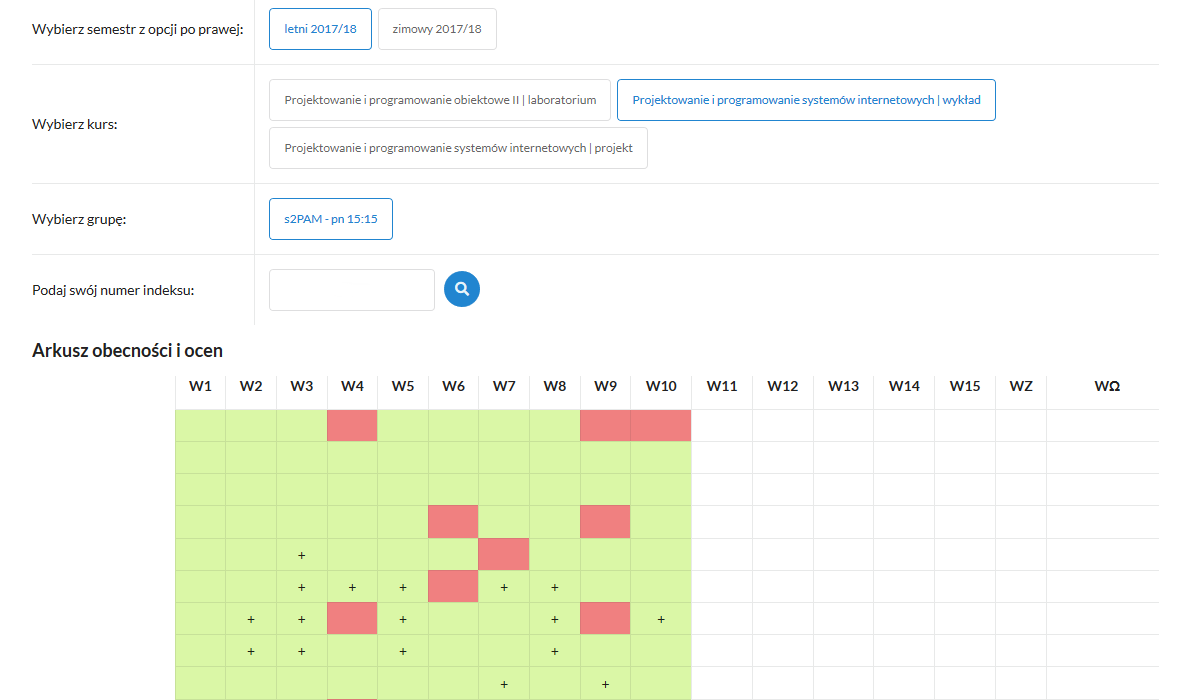
\includegraphics[width=\linewidth]{oceny.png}
	\end{figure}
\end{frame}

\begin{frame}{Pod maską}
	\begin{figure}[t]
		\centering
		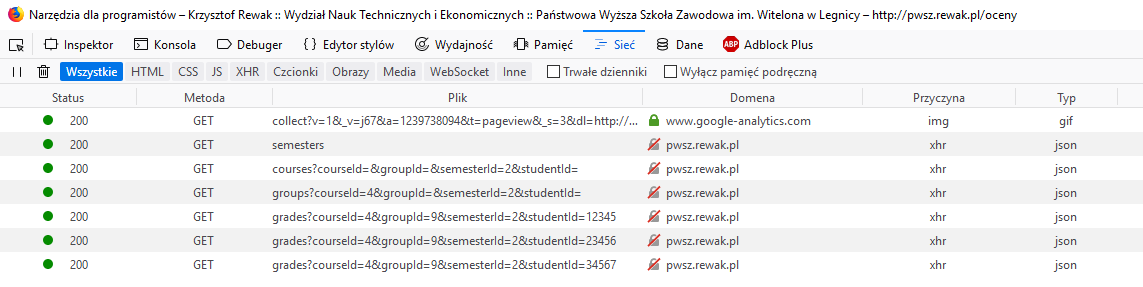
\includegraphics[width=\linewidth]{f12.png}
	\end{figure}
\end{frame}

\begin{frame}{Przypływ klasyczny}
	Okazuje się, że czasami zapytanie do serwera nie wymusza przeładowania bieżącej strony. Wówczas najczęściej mówimy o technologii AJAX.
\end{frame}

\section{AJAX}

\begin{frame}{Ajax? Francis?}
	\textbf{AJAX} (ang. \emph{Asynchronous JavaScript and XML}), czyli asynchroniczny JavaScript i XML, to technika wykorzystywana przy asynchronicznym odpytywaniu serwera od strony klienta.
\end{frame}

\begin{frame}{AJAX w praktyce}
	Idea jest bardzo podobna jak przy odpytywaniu klasycznym:
	\begin{itemize}
	\item klient wysyła zapytanie na serwer
	\item zapytanie jest przetwarzane
	\item klient odbiera odpowiedź serwera
	\end{itemize}
\end{frame}

\begin{frame}{AJAX w praktyce}
	Róznica polega na tym, że zapytanie nie jest przeładowaniem URL strony, a przesyłane jest \emph{w tle}.
	
	Użytkownik pozostaje zatem w tym samym miejscu, w którym był oraz może wchodzić w dalsze interakcje z serwisem.
\end{frame}

\begin{frame}{Zalety}
	Wykorzystanie technologii AJAX ma wiele zalet. 
	
	Wszystkie zostaną przedstawione na przykładach znanego studentom internetowego systemu dla prowadzących zajęcia.
\end{frame}

\begin{frame}{Zaleta \emph{uno}}
	Oto lista kursów w CRUD-owej tabelce:
	\begin{figure}[t]
		\centering
		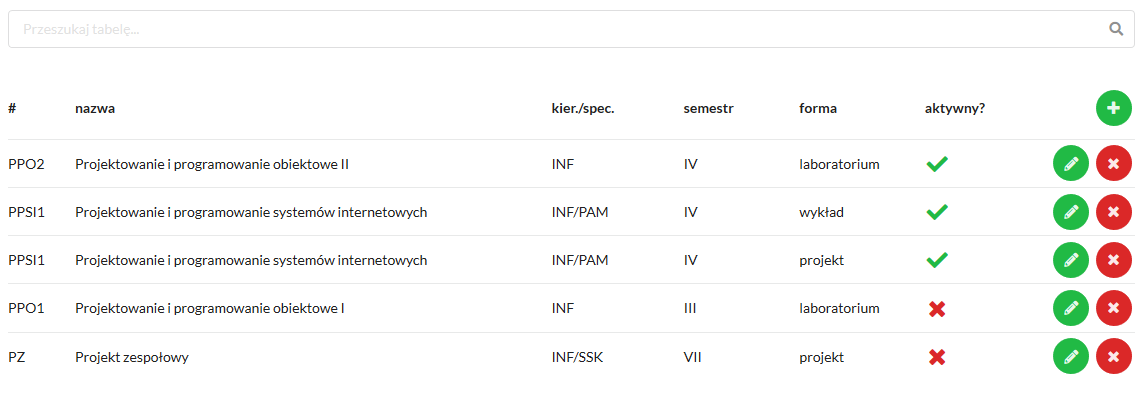
\includegraphics[width=\linewidth]{kursy.png}
	\end{figure}
	
	(CRUD to skrótowiec od \emph{create, read, update and delete})
\end{frame}

\begin{frame}{Zaleta \emph{uno}}
	Jeżeli okna edycji i potwierdzenie usunięcia otwierałyby się w oknach modalnych, wówczas prymitywne rozwiązanie polegałoby na wygenerowaniu $n + n$ różnych zestawów danych dla każdego z $n$ rekordów.
	
	Można też podłączyć zdarzenie na kliknięcie przycisku \emph{edytuj} do metody, która wywoła asynchronicznie pobranie informacje na temat edycji. Wówczas ograniczymy kod do stworzenia dwóch okien modalnych, które będą \emph{w locie} wypełniane tylko dla wybranego przypadku.
\end{frame}

\begin{frame}{Zaleta \emph{uno}}
	Zaleta numer jeden:
	
	Można zmniejszyć rozmiar i redundancję (nawet generowanego) kodu.
\end{frame}

\begin{frame}{Zaleta \emph{due}}
	Oto arkusz ocen i obecności dla wybranej grupy:
	\begin{figure}[t]
		\centering
		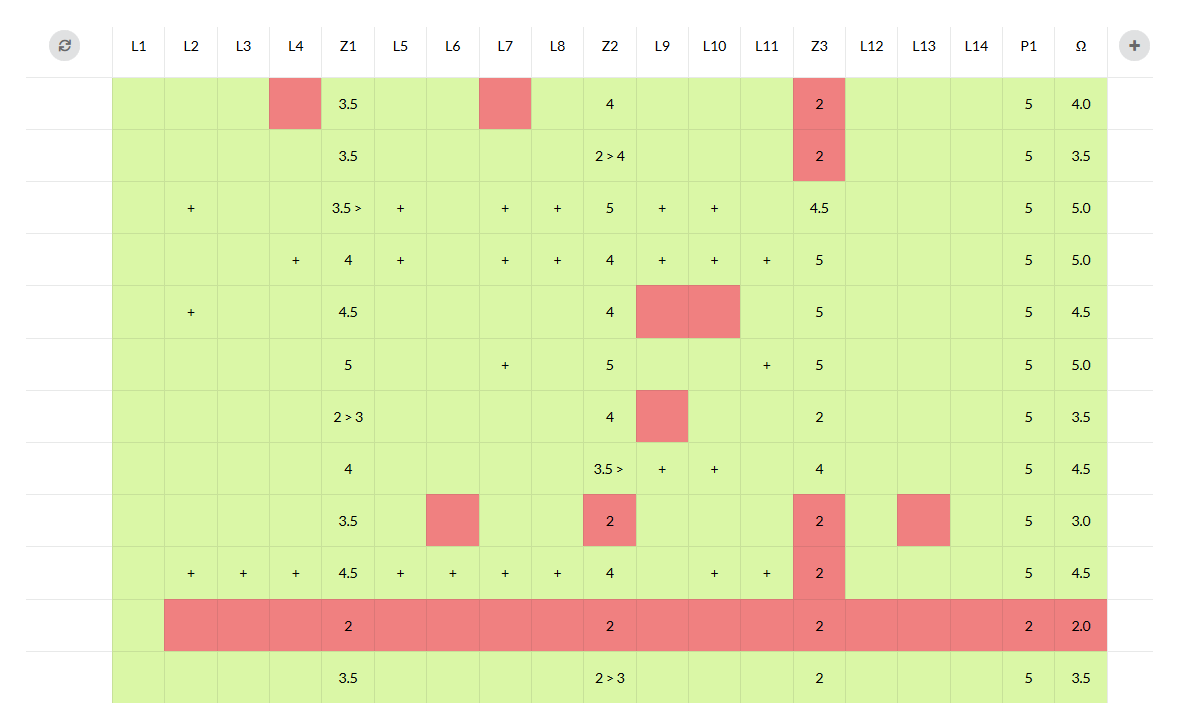
\includegraphics[width=\linewidth]{oceny-edytor.png}
	\end{figure}
\end{frame}

\begin{frame}{Zaleta \emph{due}}
	W tradycyjnym przepływie zapytań istniałyby dwie opcje: wysłanie całego arkusza naraz lub wysyłanie każdej oceny i obecności osobno. Pierwsze rozwiązanie byłoby bardzo podatne na pomyłki, a drugie - przeraźliwie powolne.
	
	Można też podłączyć zdarzenie na dwuklik lub wciśnięcie klawisza \emph{enter} w wybranej komórce oceny do metody, która wywoła asynchronicznie wysłanie informacji do backendu. Wówczas oceny będą przesyłane pojedynczo, ale bez zbędnego oczekiwania na przeładowanie strony.
\end{frame}

\begin{frame}{Zaleta \emph{due}}
	Zaleta numer dwa:
	
	Można zmniejszyć możliwość popełnienia błędu oraz zwiększyć szybkość korzystania z systemu internetowego. Inaczej: ulepszamy UX, \emph{user experience}.
\end{frame}

\begin{frame}{Zaleta \emph{tre}}
	Oto struktura folderów projektu:
	\begin{figure}[t]
		\centering
		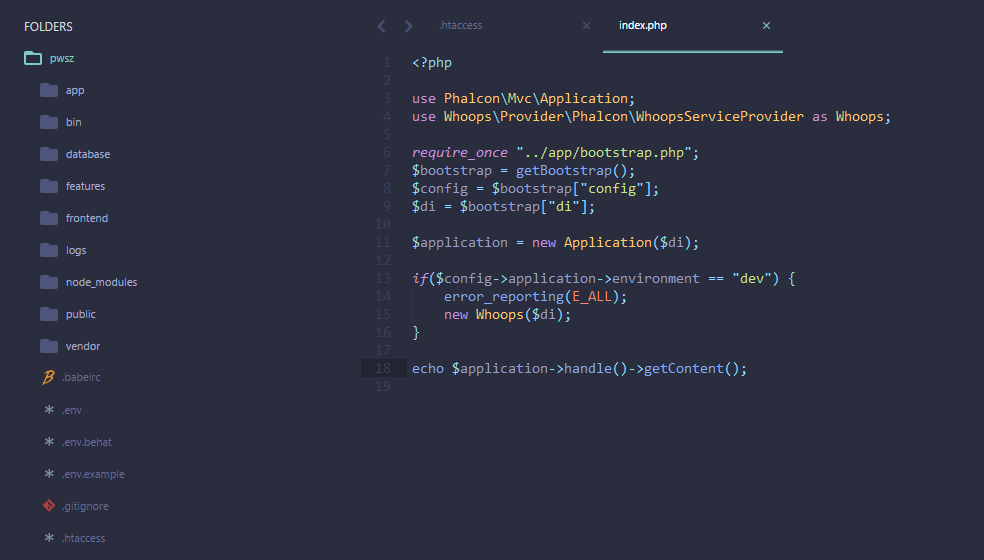
\includegraphics[width=\linewidth]{foldery.png}
	\end{figure}
\end{frame}

\begin{frame}{Zaleta \emph{tre}}
	Tworząc klasyczną aplikację internetową, przynajmniej jeden programista musi znać zarówno technologie frontendowe i backendowe. Ponadto kontrolery najczęściej zwracająca całe widoki, więc frontend jest uzależniony od backendu.
	
	Korzystając z asynchronicznych zapytań można całkowicie oddzielić frontend od backendu. W przedstawionym przykładzie widać to na podziale na foldery \texttt{app} i \texttt{frontend}, ale mogą to być całkowicie osobne repozytoria, projekty i serwery.
\end{frame}

\begin{frame}{Zaleta \emph{tre}}
	Zaleta numer trzy:
	
	Można odseparować warstwy aplikacji i przekazywać jedynie istotne dane.
\end{frame}

\begin{frame}{A wady?}
	Korzystanie z asynchronicznych zapytać oczywiście ma swoje wady:
	\begin{itemize}
	\item klient musi mieć włączoną obsługę JavaScriptu (ale kto jej teraz nie ma?),
	\item robotom z wyszukiwarek ciężej przeskanować taką witrynę (ale to można obejść tworząc mapę strony),
	\item zaburzony zostaje klasyczny przepływ ruchu na stronie internetowej, więc niektórzy użytkownicy mogą poczuć się zrezorientowani (co można oprogramować dodatkowo, \emph{vide} router SPA na mojej stronie).
	\end{itemize}
\end{frame}

\section{Przykłady}

\begin{frame}[fragile]{Vanilla JavaScript}
	Korzystając z czystego JavaScriptu można napisać następująco:
	
	\begin{lstlisting}
var xhr = new XMLHttpRequest();

xhr.open("GET", "/api/courses");

xhr.onreadystatechange = function() {
    console.log(xhr.responseText);
}

xhr.send(null);
	\end{lstlisting}
\end{frame}

\begin{frame}[fragile]{jQuery}
	Analogiczne zapytanie z wykorzystaniem popularnej biblioteki jQuery może wyglądać następująco:
	
	\begin{lstlisting}
$.ajax({
    type: "GET",
    url: "api/courses",
    success: function(data) {
        console.log(data);
    },
    error: function() {
        console.log("Error");
    }
});
	\end{lstlisting}
\end{frame}

\begin{frame}[fragile]{JavaScript API}
	Ponadto istnieje funkcja \texttt{fetch} korzystająca z javascriptowych obietnic:
	
	\begin{lstlisting}
fetch("api/courses").then(function(response) {
    return response.text();
}).then(function(data) {
    console.log(data);
}).catch(function(error) {
    console.log("Error: " + error);
});
	\end{lstlisting}
\end{frame}

\begin{frame}{Nowoczesne frameworki}
	Pobieranie danych asynchronicznie jest podstawą działania współczesnych frameworków frontendowych.
	
	Angular, React czy Vue są popularnymi rozwiązaniami, które często i coraz częściej są wykorzystywane przy budowaniu nowoczesnych systemów internetowych.
\end{frame}

\begin{frame}{Nowoczesne frameworki}
	Oto przykład strony z FAQ jako kompnent Vue:
\end{frame}

\begin{frame}[fragile]{FAQ.vue}	
	\begin{lstlisting}
<template>
  <div id="faq">
    <h1>FAQ</h1>

    <div class="question" v-for="question in questions">
      <div class="ui divider"></div>
      <h3 class="ui header">
        <i class="question circle outline icon"></i>
        {{ question.question }}
      </h3>
      <blockquote v-html="question.answer"></blockquote>
    </div>
  </div>
</template>
	\end{lstlisting}
\end{frame}

\begin{frame}[fragile]{FAQ.vue}	
	\begin{lstlisting}
<style scoped>
  blockquote { padding: .5em; }
  .question:first-of-type > .ui.divider { display: none; }
  .question { padding: .5em 0; }
</style>
	\end{lstlisting}
\end{frame}

\begin{frame}[fragile]{FAQ.vue}	
	\begin{lstlisting}
<script type="text/javascript">
  export default {
    data() {
      return {
        questions: [],
      }
    },
    created() {
      this.fetchInitialData()
    },
    methods: {
      fetchInitialData() {
        this.$http.get("faq").then(function(response) {
          this.questions = response.body.data
        })
      },
    },
  }
</script>
	\end{lstlisting}
\end{frame}

\begin{frame}{\texttt{GET /api/faq}}
	\begin{figure}[t]
		\centering
		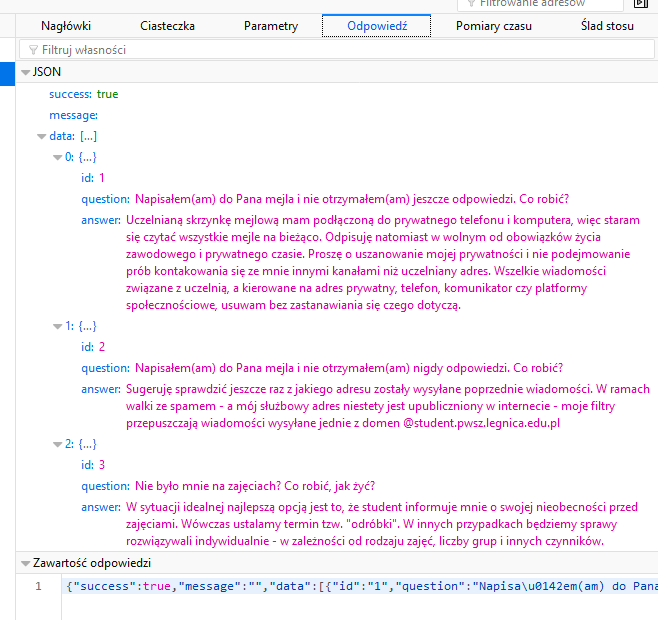
\includegraphics[width=.75\linewidth]{faq.png}
	\end{figure}
\end{frame}

\begin{frame}{I wynik!}
	\begin{figure}[t]
		\centering
		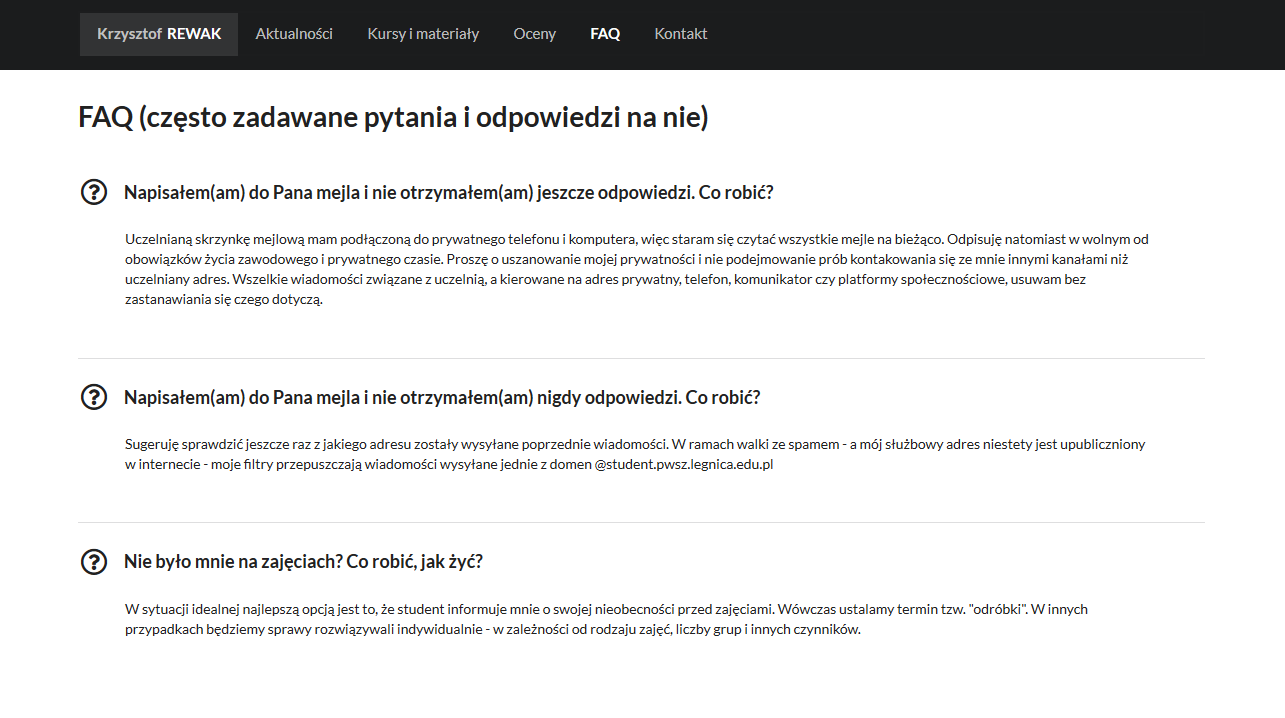
\includegraphics[width=\linewidth]{faq2.png}
	\end{figure}
\end{frame}

\section{Podsumowanie}

\begin{frame}{Bibliografia i ciekawe źródła}
  
	\begin{thebibliography}{9}
		
		\bibitem{vanilla}
		\url{https://www.sitepoint.com/guide-vanilla-ajax-without-jquery/}
		
		\bibitem{jquery}
		\url{http://api.jquery.com/jquery.ajax/}
		
		\bibitem{vue}
		\url{https://vuejs.org/v2/guide/index.html}
		
	\end{thebibliography}

\end{frame}

\appendix

\begin{frame}[standout]
	Pytania?
\end{frame}

\begin{frame}{}

	Kod prezentacji dostępny jest w repozytorium git pod adresem \texttt{https://bitbucket.org/krewak/pwsz-ppsi} \\ \ \\

	\begin{figure}
		\centering
		\href{https://bitbucket.org/krewak/pwsz-ppsi}{
			
\includegraphics[width=.15\textwidth]{../_template/bitbucket.png}
		}
	\end{figure}
	
	Wszystkie informacje dot. kursu dostępne są pod adresem \texttt{http://pwsz.rewak.pl/kursy/4} \\ \ \\

	\begin{figure}
		\centering
		\href{http://pwsz.rewak.pl/kursy/3}{
			
\includegraphics[width=.15\textwidth]{../_template/rewak.png}
		}
	\end{figure}

\end{frame}

\end{document}
